\documentclass[fontsize=12pt,paper=A4,abstract=true]{scrreprt}
\usepackage[utf8]{inputenc}
\usepackage[T1]{fontenc}
\usepackage[UKenglish]{babel}
\usepackage[backend=biber]{biblatex}
\usepackage{microtype}
\usepackage{amsmath}
\usepackage{amssymb}
\usepackage{mathtools}
\usepackage{pifont}
%\usepackage{lmodern}
\usepackage{baskervald}

%\usepackage{libertineRoman}  % TODO: remove
\usepackage{graphicx}
\usepackage{hyperref}
\usepackage{scrpage2}
\usepackage[xindy]{glossaries}
\usepackage{listings}
\usepackage[normalem]{ulem}
\usepackage{makeidx}
\usepackage{multicol}
\usepackage{caption}
\usepackage{subcaption}
\usepackage{rotating}
\usepackage{xcolor}
\usepackage[ruled,vlined]{algorithm2e}
\addbibresource{thesis.bib}

\setcounter{secnumdepth}{3}
\setlength{\parskip}{\baselineskip}
\definecolor{contr}{RGB}{180,40,0}

% Other titles:
%  1. SAT solvers in cryptanalysis
%  2. Assumption-based hash collision search in differential cryptanalysis using SAT solvers
\title{
  Using SAT Solvers to Detect Contradictions
  in Differential Characteristics
}

\author{Lukas Prokop}
\date{\today}

\makeglossaries
\makeindex

\makeatletter
\hypersetup{
  pdftitle={\@title},
  pdfauthor={\@author},
  pdfsubject={SAT solvers in cryptanalysis},
  pdfcreator={\LaTeX},
  pdfkeywords={SAT solver, hash algorithms, differential cryptanalysis},
  urlcolor=[rgb]{0.2,0.2,0.2},
  linkcolor=[rgb]{0.2,0.2,0.2},
  citecolor=[rgb]{0.1,0.1,0.1},
  baseurl={http://lukas-prokop.at/proj/bakk_iaik},
  pdfview=FitV,
  pdflang={en-US},
  unicode,
  breaklinks,
  colorlinks,
  bookmarks
}
\makeatother

\newcommand{\nltool}{nltool}
\newcommand{\cmsat}{cryptominisat}
\newcommand{\yes}{\ding{51}}
\newcommand{\no}{\ding{55}}
\newcommand{\bc}[1]{#1}  % BitCondition
\newcommand{\abs}[1]{\lvert #1\rvert}
\newcommand{\lifetime}[2]{*\,#1 \dag\,#2}
\renewcommand{\implies}{\rightarrow}

%\newcommand{\diffchar}[1]{\mbox{\ttfamily #1\obeylines}}
\newenvironment{diffchar}{\center\begingroup\ttfamily}{\endgroup\endcenter}

\newacronym{sat}{SAT}{satisfiability}
\newacronym{cnf}{CNF}{Conjunctive Normal Form}
\newacronym{dnf}{DNF}{Disjunctive Normal Form}
\newacronym{csp}{CSP}{Constraint Programming}

\makeatletter
\def\UL@putbox{\ifx\UL@start\@empty \else % not inner
  \vrule\@width\z@ \LA@penalty\@M
  {\UL@skip\wd\UL@box \UL@leaders \kern-\UL@skip}%
    \phantom{\box\UL@box}%
  \fi}
\makeatother

\begin{document}
\newcommand{\myhref}[3][blue]{\href{#2}{\color{#1}{#3}}}%
\makeatletter
\def\@maketitle{%
  \newpage
  \thispagestyle{empty}
  \null
  \vskip 2em%
  \begin{center}%
  \let \footnote \thanks
    {\Large\bfseries Using SAT Solvers to Detect \\ Contradictions in Differential Cryptanalysis \par}%
    \vskip 1.5em%
    {\normalsize
      \lineskip .5em%
      \begin{tabular}[t]{c}%
        \@author \\
        <\href{mailto:lukas.prokop@student.tugraz.at}{\color{contr}{lukas.prokop@student.tugraz.at}}> \\
        \vspace{260pt} \\
        Advisors: Florian Mendel, Martin Schläffer \\[12pt]
        
\includegraphics{img/iaik.pdf} \\[12pt]
        Institute for Applied Information \\ Processing and Communications, TU Graz, Austria \\
      \end{tabular}\par}%
    \vskip 1em%
    {\normalsize Dated: \@date}%
  \end{center}%
  \par
  \vskip 1.5em}
\@maketitle
\makeatother


\newpage
\subsection*{\centerline{Statement of Originality}}
%
\vspace{14pt}\indent
This thesis contains no material that has been accepted for the recognition
of any other degree at any other university. To the best of my knowledge,
this thesis contains no material previously published or written
by another person, except where reference is made in the text.
\vspace{30pt}

\noindent\uline{--- Lukas Prokop ---} \\[5pt]
\phantom{---} Lukas Prokop \phantom{---}

\begingroup
\hypersetup{colorlinks=true,linktoc=all,linkcolor=contr}
\tableofcontents
\endgroup

\begin{abstract}
  The NP-completeness of SAT has been proven in 1971 by Stephen Cook
  and under the assumption of $P \neq N\!P$, the problem is infeasible
  for large problem sizes. However, recent advances in the field of
  SAT solver design make large SAT problems solvable on an industrial
  level if enough computational resources are provided.
  At the same time, hash algorithms' collision resistance depends
  on the computational complexity of the algorithm which has successfully
  been reduced by Wang~et~al.
  Combining those techniques we might be able break the security of
  modern hash algorithms.
  In this bachelor's thesis we present an implementation for performing
  (partial) SAT-based attacks on hash algorithms by evaluating the
  satisfiability of differential characteristics. We evaluate three
  possible CNF encodings for this problem.
\end{abstract}

\chapter{Introduction}
\label{chap:introduction}
Hash algorithms are ubiquitous in our world of digital communication.
For example using hash algorithms we can verify data integrity of messages
with high probability without transmitting the actual message. Fundamentally
hash algorithms take arbitrary input data and return a hash value of fixed
size specific for this input. In cryptology the security of cryptographic
systems depends on three properties of hash algorithms. One of them is called
collision resistance meaning that given a hash value it is computationally
infeasible to find two different inputs leading to the defined hash value.

SAT solvers are sophisticated tools to solve difficult mathematical problems
in the most efficient way. They take a boolean equation as input and tell
whether or not the logical system is consistent or not. This way it can tell
whether a particular state of the system is desirable or not; once it is
represented with boolean algebra.

In this bachelor's thesis we combine both ideas. We will use SAT solvers to
represent states in the hash algorithm evaluation. Given an intermediate
state of the evaluation, we consider additional assumptions which might
lead to the representation of a hash collision. We can use our implementation
to verify whether this assumption is a valid state within the hash algorithm
specification. This way we are searching for collisions within the hash
algorithm starting with an intermediate state.

Our implementation is an extension of an existing framework for differential
cryptanalysis. We therefore do not represent the state of an hash algorithm
evaluation directly, but rather the difference between two instances evaluating
a hash algorithm. Hopefully each instance will end up with different input data
but the same hash value.

We introduce three encodings to represent the differential state in boolean
algebra to build a bridge between SAT solving and hash algorithm cryptanalysis.


\chapter{Automated search for differential characteristics}
\label{chap:search}
\section{Cryptographic hash algorithms}
\label{sec:hashalgs}
%
\index{Preimage resistance}
\index{Second-preimage resistance}
\index{Collision resistance}
A hash algorithm is a function assigning a given key to a value of fixed width $n$. Formally we define a hash function as $h: \{0, 1\}^* \rightarrow \{0, 1\}^n$. Hash functions in cryptography have to fulfill three requirements%
~\cite[2]{Cry02}:
%
\begin{description}
  \item[Preimage resistance] It is computationally infeasible to find a preimage
    $x$ for any given $y$ such that $h(x) = y$.
  \item[Second-preimage resistance] It is computationally infeasible to find a
    second preimage $x'$ for any given $x$ such that $h(x) = h(x')$ with $x \neq x'$.
  \item[Collision resistance] It is computationally infeasible to find two preimages
    $x$ and $x'$ for any given output $y$ such that $h(x) = h(x') = y$ with $x \neq x'$.
\end{description}

\section{SAT-based attacks}
\label{sec:sat_attacks}
%
% REMARK: https://github.com/vegard/sat2013-cryptocompo
Every year new \gls{sat} solvers in the \gls{sat} competition~\cite{Sat21} emerge and use new techniques to improve upon solving problems in real-world applications, combinatorial hard and random problems.

SAT-based attacks on cryptographic hash functions describe the approach to represent a hash function in \gls{cnf} and solve the equation system with a \gls{sat} solver to look for preimages and collisions. Prior work in this field was done including:

\index{XOR clauses}
\begin{itemize}
  \item
Ekawat Homsirikamol, Paweł Morawiecki, Marcin Rogawski and Marian Srebrny~\cite{Cry04} evaluated the security margin of SHA-3 candidates. On the one hand they applied brute-force attacks to perform preimage attacks\footnote{The authors point out that an easy modification leads to a second preimage or collision attack.} and on the other hand they compare the number of broken rounds to the total number of rounds in the given cryptographic system. The first task can be subdivided into 3 parts: Generation of the CNF formula, fixing the hash and its padding bits in the formula and running a \gls{sat} solver on the generated CNF. They conclude that all five SHA-3 contest finalists have substantially bigger security margins than the SHA-256 and SHA-1 standards in regards of SAT-based attacks.
  \item
A paper ``Extending SAT Solvers to Cryptographic Problems'' by Mate Soos, Karten Nohl and Claude Castelluccia~\cite{Cry06} builds the foundation of \cmsat{}; the \gls{sat} solver used in this bachelor's thesis. It describes a possible extension of the input algebra for XOR operations. Cryptographic primitives often use XOR operations and the authors expect performance improvements for SAT-based attacks using Gaussian elimination. \cmsat{}~2.9.10 was used in our implementation which natively uses \emph{XOR clauses}. However the \cmsat{} 3.0 release discards XOR clauses, because research in this field did not take off.
  \item
Dejan Jovanović and Predrag Janičić~\cite{Sat03} described a framework to transform a hash algorithm implementation into a SAT problem instance. They use C++'s operator overloading to replace the semantics of the operators with the corresponding boolean ones. When transforming the problem into a CNF, they used Tseitin's Definitional Normal Form with linear growth of size rather than an exponential approach which is taken in this thesis. They concluded that a whole MD4 or MD5 instance cannot be evaluated with their implementation, but the problem can be scaled down by reducing the size of the input message or reducing the number of rounds. The paper has a very similar motivation, but this thesis targets differential cryptanalysis.
\end{itemize}

\section{Differential cryptanalysis}
\label{sec:differential}
\index{Differential cryptanalysis}
%
\begin{figure}[t]
  \begin{center}
    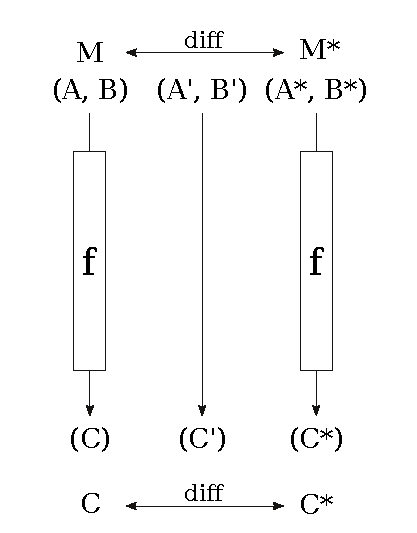
\includegraphics{img/diff_cryptanalysis.pdf}
    \caption{Two evaluation instances in differential cryptanalysis and their difference.}
    \label{fig:diff_cryptanalysis}
  \end{center}
\end{figure}

\index{Evaluation instances}
In \emph{differential cryptanalysis} we consider the difference between \emph{evaluation instances}. Assuming a hash function $f$ maps some input $M$ (derived from two parameters $A$ and $B$) to some output $C$, the difference between those instances in every step of the evaluation of the function $f$ is of interest for us. In Figure~\ref{fig:diff_cryptanalysis} an example with two instances $M$ and $M^*$ is illustrated.

Xiaoyun Wang successfully reduced the complexity of MD4, the original RIPEMD design and MD5 in 2005~\cite{Cry10} which made differential cryptanalysis popular in the research community.

In our thesis we want to discuss how differential characteristics can be encoded in boolean algebra. Fabio Massacci was the first to apply SAT research to cryptographic problems and coined the name \emph{logical cryptanalysis}. Our implementation specifically combines the fields of differential cryptanalysis and logical cryptanalysis.

In all following sections we always assume \emph{two} existing evaluation instances.

\subsection{Differential characteristics}
\label{sec:differential-characteristic}
%
In the following we want to describe a notation introduced by Christophe De Cannière and Christian Rechberger in their paper ``Finding SHA1-Characteristics: General Results and Applications''~\cite{Cry01}.

With our notation we want to represent the difference of single bits in those instances. In general 4 ($= 2^2$) cases must be distinguished, because of 2 values for 2 bits.

But in differentical cryptanalysis we often do not have enough information about the bits. We need to model insecurity. For example if the first bit is a zero, but the value of the second bit is unknown, 2 cases are possible ($0$ and $0$/$1$ for the first and second bit respectively). If we want to model ``the bits are different'' 2 cases are possible again. However if no knowledge about the bits' state is available, we have to consider all 4 cases.

\index{Bit condition}
\index{Free bit condition}
\index{Contradiction}
For the general notation we have to scale this picture. We have one bit in each evaluation instance and some of four different states are possible. This gives us 16 cases to distinguish: 1 case where no bit configuration is possible (the so-called \emph{contradiction}), 4 cases where only one configuration is possible, 6 cases with 2 configurations, 4 cases with 3 configurations and 1 configuration where every configuration is possible (the so-called \emph{free condition}). These cases are listed in Table~\ref{tab:bitconditions}. The most-left column specifies the so-called \emph{bit condition} representing a differential value. The superset relation between the bit conditions can be retrieved from the Galois lattice given in Figure~\ref{fig:bitconditions-lattice}.

% TODO: urgh, \yes and \no must not be bold. Or whatever to make the table beautiful
\begin{table}[p]
 \begin{center}
  \begin{tabular}{ccccc}
   \hline
    $(X_i, X_i^*)$ & (0, 0) & (1, 0) & (0, 1) & (1, 1) \\
   \hline \hline
         ?         & \yes   & \yes   & \yes   & \yes   \\
         -         & \yes   & \no    & \no    & \yes   \\
         x         & \no    & \yes   & \yes   & \no    \\
         0         & \yes   & \no    & \no    & \no    \\
         u         & \no    & \yes   & \no    & \no    \\
         n         & \no    & \no    & \yes   & \no    \\
         1         & \no    & \no    & \no    & \yes   \\
         \#        & \no    & \no    & \no    & \no    \\
         3         & \yes   & \yes   & \no    & \no    \\
         5         & \yes   & \no    & \yes   & \no    \\
         7         & \yes   & \yes   & \yes   & \no    \\
         A         & \no    & \yes   & \no    & \yes   \\
         B         & \yes   & \yes   & \no    & \yes   \\
         C         & \no    & \no    & \yes   & \yes   \\
         D         & \yes   & \no    & \yes   & \yes   \\
         E         & \no    & \yes   & \yes   & \yes   \\
   \hline
  \end{tabular}
  \caption[Bit conditions table]{Bit conditions table (most-left column specifies symbol).}
  \label{tab:bitconditions}
 \end{center}
\end{table}
\begin{figure}[p]
 \begin{center}
  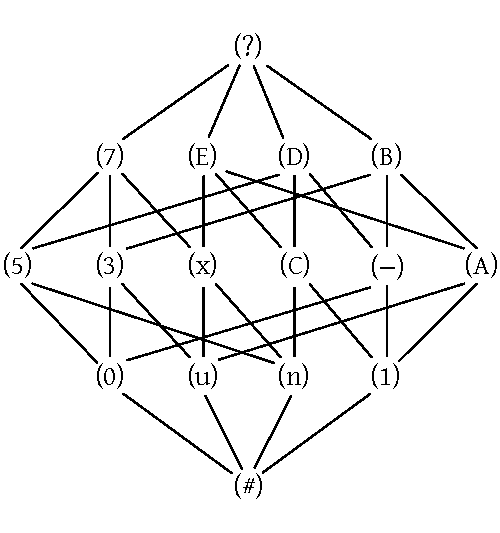
\includegraphics{img/bit_condition_lattice.pdf}
  \caption{Galois lattice of bit conditions.}
  \label{fig:bitconditions-lattice}
 \end{center}
\end{figure}

\index{Differential characteristic}
\index{Bitslice}
\index{Differential word}
In conclusion we introduced a notation to describe which bit configurations for two bits are possible in a certain state. A \emph{differential characteristic} represents a certain state of a hash algorithm in differential cryptanalysis. It is a list of bit conditions often represented as a matrix for better readability. A \emph{bitslice} is a column in a given differential characteristic. Analogously a \emph{differential word} is a row in a given differential characteristic.

\section{Evaluating differential characteristics}
\label{sec:diffchar-examples}
%
Several popular hash algorithms are built using the ARX architecture\footnote{The MD5, SHA-1 and SHA-2 hash algorithms follow the ARX design principle.}. One of the letters in the name refers to the XOR operation taking two or more arguments. The XOR operator returns true iff the number of arguments with value true is odd.

Let's consider a single bitslice with 2 input arguments and 1 output argument. The first input argument is \bc{1} and the second input argument is \bc{0}. It's important that \bc{1} and \bc{0} are bit conditions and therefore describe the state of 2 instances. For these particular bit conditions the values of both instances are the same: 1 and 0 respectively.
%
\begin{figure}[t]
  \begin{center}
    \begin{subfigure}[b]{0.23\textwidth}
      \begin{diffchar}
        A: 1 \\
        A: 0 \\
        S: 1
      \end{diffchar}
      \caption{SAT}
      \label{dc:xor1}
    \end{subfigure}%
    \begin{subfigure}[b]{0.23\textwidth}
      \begin{diffchar}
        A: 1 \\
        A: 0 \\
        S: ?
      \end{diffchar}
      \caption{SAT}
      \label{dc:xor2}
    \end{subfigure}%
    \begin{subfigure}[b]{0.23\textwidth}
      \begin{diffchar}
        A: 0001 \\
        A: 1010 \\
        S: 1011
      \end{diffchar}
      \caption{SAT}
      \label{dc:xor3}
    \end{subfigure}%
    \begin{subfigure}[b]{0.23\textwidth}
      \begin{diffchar}
        A: C\textendash{}\textendash{}? \\
        A: 3xx0 \\
        S: x?x?
      \end{diffchar}
      \caption{SAT}
      \label{dc:xor4}
    \end{subfigure}
    \caption{Examples for satisfiable differential characteristics (XOR operation).}
    \label{dc:xor-examples}
  \end{center}
\end{figure}
\begin{figure}[t]
  \begin{center}
    \begin{diffchar}
      A: BC0 \\
      A: 501 \\
      S: \textendash{}10
    \end{diffchar}
    \caption{An unsatisfiable differential characteristic (XOR operation).}
    \label{dc:xor-faulty}
  \end{center}
\end{figure}
%
Figure~\ref{dc:xor-examples} shows examples for satisfiable differential characteristics. If we apply the XOR operation on each bitslice, the output value does correspond to the given bit condition. Correspondence here means that any possible outcome of the function is part of the specified output argument. It is the hash algorithm's responsibility to define which arguments an operation is applied to. Here we assume a simple algorithm which applies XOR bitslice-by-bitslice.

In Figure~\ref{dc:xor1} a one as result in both instance is satisfiable for the XOR operation. In Figure~\ref{dc:xor2} we also have a satisfiable result, because \bc{?} is a superset of \bc{1}. Figure~\ref{dc:xor3} just illustrates the simultaneous application of the XOR operation to each bitslice of the differential characteristic. Figure~\ref{dc:xor4} provides more complex examples. For the second bitslice (from the right) the XOR operation applied to an input argument of equal values in both instances and an input argument with different values, the result will always be a difference between both instances. The third bitslice shows again a superset relation between \bc{?} and \bc{x}. In the fourth bitslice we also have to distinguish 4 cases (\bc{C} and \bc{3} can be 2 cases each) and if we evaluate the result, the bits in both instances will always be different.

A bit condition taken twice as input arguments to XOR is always \bc{0}. If a contradiction occurs in an input argument, the result is a contradiction. In Figure~\ref{dc:xor-faulty} an unsatisfiable differential characteristic is given. It is unsatisfiable, because some application of the XOR operation does not result in the specified bit condition; actually all applications will fail. The second bitslice is unsatisfiable, because if \bc{C} represents a 0 in the first instance and a 1 in the second instance, the application of XOR will return a 0 and 1 in each instance respectively which is not covered by the bit condition \bc{1}. The third bitslice has two input arguments which actually allows any possible result and relation between the values in each instance. Thus the bit condition \bc{-} is too strict.

Evaluating the satisfiability of a differential characteristic is the main requirement to enable our automated search.

\section{\nltool}
\label{sec:nltool}
%
\nltool{} is a framework for differential cryptanalysis. It provides various hash algorithm implementations and also allows to run partial subsets (like steps or rounds as defined by the particular hash algorithm). It implements a search algorithm trying to derive knowledge about some differential state of the hash algorithm evaluation. This propagation is a crucial task of the tool and this implementation improves upon existing ones. The tool and the details of the search got introduced in the paper~\cite[293]{Cry07}. For our implementation it is important to distinguish between two states within the search:

\begin{description}
  \item[Initialization]
    At initialization the hash algorithm (to be used) is known and the structure of the differential characteristic can be retrieved. The value of any bit condition is not yet available.
  \item[Update BitCondition]
    In the update step the values of the differential characteristic are provided and the final decision about satisfiability of the characteristic can be made.
\end{description}

Finding the best paths to derive new knowledge about the state is an open research topic. Differential paths are described in the master thesis ``Cryptanalysis of MD4'' by Martin Schläffer~\cite{Cry15} and an application of the tool for an attack is given by the paper ``Collision Attacks on the Reduced Dual-Stream Hash Function RIPEMD-128''~\cite{Cry08}.

\section{Automated search}
\label{sec:automated-search}
%
The search strategy applied to SHA-256 is a more sophisticated version than the one proposed by~\cite[10]{Cry01} and was proposed in the paper ``Finding SHA-2 Characteristics: Searching Through a Minefield of Contradictions''~\cite[298]{Cry07}:
\begin{quote}
Let \emph U be the set of all \texttt{`?'} and \texttt{`x'}, then repeat the following until U is empty.
\begin{enumerate}
  \item Pick randomly a bit in in \emph U.
  \item Impose a \texttt{`-'} for a \texttt{`?'} or randomly a sign (\texttt{`u'} or \texttt{`n'}) for \texttt{`x'}.
  \item Compute the propagation.
  \item If a contradiction is detected start backtracking, else apply additional checks.
  \item Continue with step 1 if all checks passed, if not start backtracking.
  \item If the decision bit is \texttt{`x'} try the second choice of the sign or if the decision bit \texttt{`?'} impose a \texttt{`x'}
  \item If still a contradiction occurs mark bit as critical.
  \item Jump back until the critical bit ca will be resolved.
  \item Continue with step 1.
\end{enumerate}
\end{quote}

\index{Overlapping bits}
The interesting point here is that the SAT solver implementation provides better propagation results. In the initialization step the reused values are known and the SAT solver implementation only creates boolean variables for values whenever they occur the first time. \emph{Overlapping bit} detection for two-bit conditions (as mentioned in \cite[296]{Cry07}) is an improvement of \nltool{} provided in this implementation. Overlapping bits are bit conditions which are used twice in a differential characteristic (and thus within the hash algorithm). So they always have the same value.

\section{Testcases for the Addition and Sigma function}
\label{sec:add-sigma-testcases}
%
Tables~\ref{dc:tcs-addition} and \ref{dc:tcs-sha2} list various testcases for the Addition and Sigma function and their satisfiability state. The Addition function uses carry bits\footnote{Denoted by a differential word C.} whose values are used in the next bitslice and is defined by

\index{Addition function}
\begin{minipage}{0.48\textwidth}
  \begin{align*}
    s_0 &= a_0 \oplus b_0 \\
    c_1 &= a_0 \land b_0 \\
    s_1 &= a_1 \oplus b_1 \oplus c_1 \\
    c_2 &= (a_1 \land b_1) \lor (b_1 \land c_1) \lor (c_1 \land a_1)
  \end{align*}
\end{minipage}
\begin{minipage}{0.48\textwidth}
  \begin{align*}
    s_2 &= a_2 \oplus b_2 \oplus c_2 \\
    c_3 &= (a_2 \land b_2) \lor (b_2 \land c_2) \lor (c_2 \land a_2) \\
    s_3 &= a_3 \oplus b_3 \oplus c_3
  \end{align*}
\end{minipage}

The Sigma function is defined by
\index{Sigma function (SHA-2)}
\begin{align*}
    b_0 &= a_1 \oplus a_2 \oplus a_3 \\
    b_1 &= a_2 \oplus a_3 \oplus a_0 \\
    b_2 &= a_3 \oplus a_0 \oplus a_1 \\
    b_3 &= a_0 \oplus a_1 \oplus a_2
\end{align*}

and the corresponding C++ definition can be seen in Listing~\ref{lst:sigma} at page~\pageref{lst:sigma}. $a_0$ refers to the most-right value of the differential word A using zero-based indexing. $a_1$, $b_0$ and others are defined respectively.

So in conclusion both functions reuse bits of the previous bitslice. Previous implementations could not detect such \emph{overlapping bits} and this detection provides a better propagation result in the automated search, because cases where the overlapping bit condition differs must not be tested.

%Figure~\ref{fig:sigma-vis} tries to visualize the reuse of the values in the function with colors.
%
%\begin{figure}[t]
%  \begin{center}
%    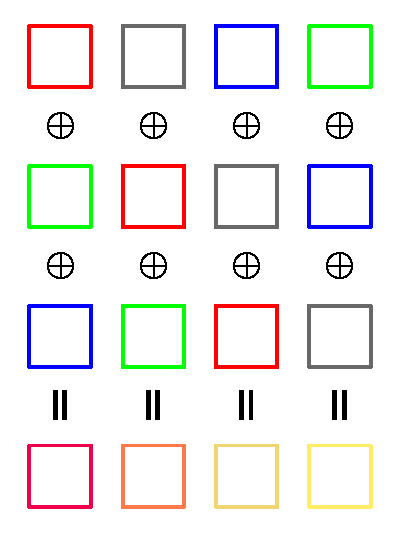
\includegraphics{img/sigma.pdf}
%    \caption{Values of the Sigma function visualized.}
%    \label{fig:sigma-vis}
%  \end{center}
%\end{figure}

\begin{figure}[p]
  \begin{center}
    \begin{subfigure}[b]{0.23\textwidth}
      \begin{diffchar}
        A: 0011 \\
        B: 0101 \\
        S: 1000
      \end{diffchar}
      \caption{SAT}
      \label{dc:tcs-addition-1}
    \end{subfigure}
    \begin{subfigure}[b]{0.23\textwidth}
      \begin{diffchar}
        A: 0011 \\
        B: 0101 \\
        S: 0000
      \end{diffchar}
      \caption{UNSAT}
      \label{dc:tcs-addition-2}
    \end{subfigure}
    \begin{subfigure}[b]{0.23\textwidth}
      \begin{diffchar}
       A: \textendash{}\textendash{}\textendash{}x \\
       B: \textendash{}\textendash{}\textendash{}x \\
       S: ???x
      \end{diffchar}
      \caption{UNSAT}
      \label{dc:tcs-addition-3}
    \end{subfigure}
    \begin{subfigure}[b]{0.23\textwidth}
      \begin{diffchar}
        A: \textendash{}\textendash{}\textendash{}x \\
        B: \textendash{}\textendash{}\textendash{}x \\
        S: ???\textendash{}
      \end{diffchar}
      \caption{SAT}
      \label{dc:tcs-addition-4}
    \end{subfigure}
  \end{center}%

  \begin{center}
    \begin{subfigure}[b]{0.23\textwidth}
      \begin{diffchar}
        A: \textendash{}\textendash{}\textendash{}x \\
        B: \textendash{}\textendash{}\textendash{}x \\
        S: ????
      \end{diffchar}
      \caption{SAT}
      \label{dc:tcs-addition-5}
    \end{subfigure}
    \begin{subfigure}[b]{0.23\textwidth}
      \begin{diffchar}
        A: \textendash{}\textendash{}\textendash{}\textendash{} \\
        B: \textendash{}\textendash{}\textendash{}x \\
        S: x\textendash{}??
      \end{diffchar}
      \caption{UNSAT}
      \label{dc:tcs-addition-6}
    \end{subfigure}
    \begin{subfigure}[b]{0.23\textwidth}
      \begin{diffchar}
        A: \textendash{}\textendash{}\textendash{}x \\
        B: \textendash{}\textendash{}\textendash{}x \\
        S: x???
      \end{diffchar}
      \caption{SAT}
      \label{dc:tcs-addition-7}
    \end{subfigure}
  \end{center}
  \caption{Testcases for the ADD2 function (addition with 2 input arguments).}
  \label{dc:tcs-addition}
\end{figure}

\begin{figure}[p]
  \begin{center}
    \begin{subfigure}[b]{0.23\textwidth}
      \begin{diffchar}
        A: \textendash{}\textendash{}\textendash{}\textendash{} \\
        S: 0000
      \end{diffchar}
      \caption{SAT}
      \label{dc:tcs-sigma-1}
    \end{subfigure}
    \begin{subfigure}[b]{0.23\textwidth}
      \begin{diffchar}
        A: 7C\textendash{}3 \\
        S: \textendash{}3u?
      \end{diffchar}
      \caption{SAT}
      \label{dc:tcs-sigma-2}
    \end{subfigure}
  \end{center}

  \begin{center}
    \begin{subfigure}[b]{0.23\textwidth}
      \begin{diffchar}
        A: \textendash{}\textendash{}\textendash{}x \\
        S: 0000
      \end{diffchar}
      \caption{UNSAT}
      \label{dc:tcs-sigma-3}
    \end{subfigure}
    \begin{subfigure}[b]{0.23\textwidth}
      \begin{diffchar}
        A: xxxx \\
        S: 0000 \\
      \end{diffchar}
      \caption{UNSAT}
      \label{dc:tcs-sigma-4}
    \end{subfigure}
    \begin{subfigure}[b]{0.23\textwidth}
      \begin{diffchar}
        A: 0uCD \\
        S: ADC7 \\
      \end{diffchar}
      \caption{SAT}
      \label{dc:tcs-sigma-5}
    \end{subfigure}
  \end{center}
  \caption{Testcases for the SHA-2 Sigma function.}
  \label{dc:tcs-sha2}
\end{figure}

We will discuss the differential characteristic~\ref{dc:tcs-addition-4} in more detail as an example. We have two evaluation instances and the first bitslice claims that the two input arguments for the Addition function are different between the instances. In this case the output arguments are equal. Table~\ref{tab:tcs-addition-4-first-bitslice} lists all possible cases. In any case the column $s_0$ indicates that the values in both instances are equal. Thus the bit condition \bc{-} is a valid assumption. At the same time we observe that we cannot derive much information about the state of $c_1$, which has three possible cases $(0, 0)$, $(0, 1)$ and $(1, 0)$. The case $(1, 1)$ is excluded. If we continue deducing the bit conditions for the Addition operation we observe that the carry bit makes it impossible to draw a conclusion for any $s$-value like for $s_0$. As a result this differential characteristic is valid.

\begin{table}[t]
  \begin{center}
    \begin{tabular}{l|cccc}
     \hline \hline
                 & $a_0$ & $b_0$ & $s_0$ & $c_1$ \\
     \hline
      instance 1 &   0   &   0   &   0   &   0  \\
      instance 2 &   1   &   1   &   0   &   1  \\
     \hline
      instance 1 &   0   &   1   &   1   &   0  \\
      instance 2 &   1   &   0   &   1   &   0  \\
     \hline
      instance 1 &   1   &   0   &   1   &   0  \\
      instance 2 &   0   &   1   &   1   &   0  \\
     \hline
      instance 1 &   1   &   1   &   0   &   1  \\
      instance 2 &   0   &   0   &   0   &   0  \\
     \hline \hline
    \end{tabular}
    \caption{List of possibilities for the bits of the first bitslice in Figure~\ref{dc:tcs-addition-4}.}
    \label{tab:tcs-addition-4-first-bitslice}
  \end{center}
\end{table}



\chapter{SAT solvers}
\label{chap:sat}
\section{Boolean algebra}
\label{sec:boole}
\index{Boolean algebra}
%
Boolean algebra has a long history. George Boole (\lifetime{1815}{1864}), John Venn (\lifetime{1834}{1923}) and William Stanley Jevons (\lifetime{1835}{1882}) pioneered an algebraic structure $\langle B, \lor, \land, \neg, 0, 1\rangle$ with the following properties ($x$ and $y$ are boolean expressions and therefore in $B$)~\cite[10]{Sat20}:
%
\begin{itemize}
  \item $\land$ and $\lor$ are binary operators. $\neg$ is an unary operator.
  \item $0, 1 \in B$
  \item $x \land y = y \land x; x \lor y = y \lor x$
  \item $x \lor (y \land z) = (x \lor y) \land (x \lor z); x \land (y \lor z) = (x \land y) \lor (x \land z)$
  \item $x \lor \neg x = 1; x \land \neg x = 0$
  \item $1 \land x = x; 0 \lor x = x$
\end{itemize}

In the following sections boolean algebra will be used to derive clauses for the \gls{sat} solver. De Morgan's laws are a set of transformation rules in boolean algebra of equivalent statements. The following one will be used in the document:

\[
  \neg (x \land y) \qquad\Leftrightarrow\qquad (\neg x) \land (\neg y)
\]

\section{Satisfiability}
\label{sec:sat}
\index{Satisfiability}
%
The satisfiability problem states the following question:
\begin{quote}
  ``Is a given boolean system in conjunctive normal form \emph{satisfiable}?''
\end{quote}
%
Satisfiability or consistency in logic refers to a property of a boolean expression. A boolean equation is satisfiable if and only if there exists some truth assignment for the given expression which evaluates to true.

\index{Cook-Levin theorem}
The Cook-Levin theorem states that the \gls{sat} problem is NP-complete. This was proven in 1971 by Stephen Cook~\cite{Sat01} and Leonid Levin~\cite{Sat02} independently. As such \gls{sat} problems seem to be computationally infeasible for larger problem sizes and \gls{sat} solvers are tools to solve those NP-complete problems in the best possible way.

\index{Conjunctive normal form}
\index{Disjunctive normal form}
\index{Clauses}
A $k$-SAT problem (with $k \in \mathbb{N}$) is a \gls{sat} problem in \gls{cnf} with at maximum $k$ literals per clause. A \gls{cnf} is the conjunction of disjunctions (so-called \emph{clauses}). A \gls{dnf} is the disjunction of conjunctions.

\section{SAT solving techniques}
\label{sec:satsolvers}
\index{SAT solvers}
%
\index{DIMACS format}
In 1958 Martin Davis and Hilary Putnam proposed the CNF as input for satisfiability problems in an unpublished manuscript for the NSA~\cite{Sat20}. The DIMACS format has been developed as universal input format for SAT solvers~\cite{Sat09}.

\gls{sat} solvers today are variants of the DPLL algorithm. In the original design, four techniques are discussed:
\begin{description}
  \item[Unit clause.] Clauses with one literal are immediately processed and taken as assignment. A literal is a boolean variable or its negation.
  \item[Pure literal rule.] If all occurences of a variable happen with the same polarity, all those clauses can be discarded if the variable gets assigned its polarity.
  \item[Elimination of atomic formulas.] Formulas which are atomic for the given equation system get eliminated.
  \item[Splitting rule.] Even a single variable might split the whole search space and shall be used as an advantage for speedup.
\end{description}
%
The first two techniques are explicitly part of the DPLL algorithm. The often cited paper for the DPLL algorithm is Davis' ``A Computing Procedure for Quantification Theory''~\cite{Sat05} and a discussion of the history is provided in ``Early History and Perspectives of Automated Deduction''~\cite{Sat06}. A discussion of possible approaches to this problem is given by Jun Gu, Paul W. Purdom, John Franco and Benjamin Wah~\cite{Sat08}.

Further efforts were especially put into efficient representation of the search space with techniques like early pruning, replacement of a tree-like search space with a DAG-like search space and variable choice heuristics~\cite[24]{Sat20}.

Two further rules are considered:
\begin{description}
  \item[Shortest clause rule.]
    Prefer the assignment of a variable from an existing clause containing the fewest unset literals.
  \item[Majority rule.]
    Prefer the assignment of a variable with the maximum difference between the number of its positive and negative literals.
\end{description}

\subsection{Assumptions}
\label{sec:satsolvers-assumptions}
\index{Assumptions (SAT solvers)}
%
The interface of a \gls{sat} solver typically consists of a function to add clauses and a solve function. As such most of the current \gls{sat} solvers work incrementally; they allow to add clauses to the \gls{sat} solver and to repeatedly invoke the solve function.

Assumptions are a separate concept which allows the user to specify hints. An assumption is one assignment of a variable that will be lost after one SAT solver evaluation. This way the user has a certain level of control which variables are evaluated.

Assumptions can be simply integrated to the \gls{cnf} as unit clauses if their value shall be assigned persistently.
% TODO: better research. Where are assumptions studied?

\subsection{Runtime analysis}
\label{sec:satsolvers-runtime}
%
Satisfiability of a CNF formula~$\phi$ with $n$ boolean variables can be decided in time $\mathcal{O}(2^n \abs{\phi})$ by enumerating all assignments of the variables. Also the number of literals $l$ and number of clauses $m$ have to be considered.

In 2002 researchers found some deterministic algorithm~\cite{Sat07} using local search to solve $k$-SAT instances with the best runtime to this day: $(2 - 2/(k+1))^n$. However the general \gls{sat} problem is not limited to a number of literals per clause.

Because the desired runtime is not always achieved, focus is put on the encoding and transformation of SAT instances. Grigorii Samuilovich Tseitin got famous for his research in transformations and encoding like the Tseitin encoding. In a recent paper~\cite{Sat22} Peter Stuckey points out that there are no original SAT problems and we should focus on representing problems in the way they originally appear. SAT research is closely related to the field of \gls{csp}, which also considers other encodings.

In terms of performance the following properties of a \gls{cnf} can be used as measurement~\cite{Sat20}:
\begin{description}
  \item[Encoding size.]
    is defined by the number of clauses, literals or variables.
    We always add clauses to SAT solvers making the boolean system larger. But symmetry-breaking clauses and blocked clauses can actually improve evaluation speed.
  \item[Consistency properties.]
    This includes arc consistency and forward checking.
  \item[Solution density.]
    The number of solutions divided by $2^n$ ($n$ as the number of variables). The higher the solution density, the faster a satisfying solution can be found.
\end{description}

\section{Obtain CNF and DNF from truth table}
\label{sec:cnf-dnf}
%
\index{Truth table}
Truth tables have 2 dimensions and list all possible boolean variable configurations and their outcome for a given function. Ludwig Wittgenstein established binary truth tables in his philosophical book ``Tractatus Logico-Phulosophicus''.

Having a boolean function we can always determine an equivalent \gls{cnf} or \gls{dnf}.

\begin{description}
  \item[Disjunctive normal form.]
    The disjunctive normal form can be retrieved by extracting all configurations resulting in value true. Each configuration represents a conjunction of literals. Literals are generated by taking the variable corresponding to the truth value\footnote{Value true for a variable $v$ yields the literal $v$. Value false yields the literal $\neg v$.}. The DNF is the disjunction of the configurations.
  \item[Conjunctive normal form.]
    The conjunctive normal form can be retrieved by extracting all false configurations. Each configuration represents a disjunction of literals and literals are created with opposite polarity\footnote{Value true for a variable $v$ yields the literal $\neg v$. Value false yields the literal $v$.}. The CNF is the conjunction of the configurations.
\end{description}

It is important to point out that building the truth table takes $\mathcal{O}(2^n)$ for $n$ variables if constant runtime is assumed for the evaluation of the boolean function. This leads to a problem in our implementation. In general we don't know the functions to be used in advance, but require the equivalent \gls{cnf} for the \gls{sat} solver. In our implementation we generate the truth table for every function to be used to retrieve all outcomes.



\chapter{Bridging differential cryptanalysis and SAT solving}
\label{chap:implementation}
With our implementation we want to answer the following question:
\begin{quote}
  ``Given some differential characteristic, is this characteristic satisfiable?''
\end{quote}
Equivalently is there any boolean assignment within both evaluation instances such that the applied function of the hash algorithm matches the result and the bit conditions do correspond. This question was already raised in section~\ref{sec:diffchar-examples}. This is the same question stated as main difficulty for the attack of SHA-2~\cite[293]{Cry07} when trying to apply automated search.

\section{General architecture}
\label{sec:architecture}
%
In the following we discuss various architectures to evaluate the satisfiability of differential characteristics. We try to achieve the best performance for this task within \nltool{}'s automated search.

\subsection{Hash algorithm specification and truth table}
%
At the very beginning we specify a hash algorithm. This specification contains the elementary operations. We consider some simple hash algorithm applying the SHA-2 Sigma operation consisting of XOR operations:
\lstset{language={C++},caption={A very basic hash algorithm specification},label={lst:sigma}}
\begin{lstlisting}
  satstep->Add<SatGenerator<XOR3>>(
    a->Rotr(1), a->Rotr(2), a->Rotr(3), b
  );
\end{lstlisting}

Here \texttt{satstep} is the computational unit which uses the SAT solver to report whether a given differential characteristic is satisfiable or not. \texttt{SatGenerator} is a wrapper which takes a conventional implementation like XOR of 3-digit values (manipulating values in the main memory) and creates a SAT solver equivalent for it. This is done by evaluating the truth table of the values after application of one such operation. \texttt{a} and \texttt{b} are differential words. \texttt{Rotr} rotates the given values to the right. Its number of rotations is defined in the parameter. By definition of \texttt{XOR3}, the fourth value ($\texttt{b}$) represents the result.

Every operation statically knows how many parameter it takes. The XOR3 operation takes three input parameters and one output parameter. The truth table is created once for every operation and determines which output value is generated for the given input. As such the truth table evaluation is a bottleneck in the framework due to its exponential behavior. However, a static implementation of the operation which directly adds the clauses can also be provided (thus omitting the \texttt{SatGenerator} wrapper).

Using a command line parameter \texttt{nltool} gets to know which hash algorithm to take. At this point in time, it is going to know which parameters (and their relation) are used for this hash algorithm, but not their actual values. At the same time an instance of the SAT solver is instantiated to be used later on.

The following properties are given for the primitive functions and the hash algorithm:
\begin{itemize}
  \item Any pure function using integers as arguments can be transformed into a SAT equivalent.
  \item A truth table is used exploiting exponential behavior, but this truth table generation is only run once. In a different implementation it might also run at compile time.
  \item \texttt{satstep} describes a computational unit of any scale thus allowing to combine elementary operations to advanced algebraic operations, hash algorithm rounds or even whole hash algorithms.
\end{itemize}

\subsection{Clause introduction}
\label{sec:clause-introduction}
%
Constraints to the solution of the SAT solver will be introduced in two places. The actual clauses are defined by some encoding explained in section~\ref{sec:three-approaches}:
\begin{itemize}
  \item Every bit condition is represented by a set of clauses. In our implementation we introduced a \texttt{SatCondition} object which takes a bit condition as parameter and the \texttt{addClauses} method will add all corresponding clauses to the SAT solver.
  \item The hash algorithm defines which functions are applied. This function is analyzed using a truth table and the corresponding clauses are generated.
\end{itemize}

\subsection{Structure of encodings}
\label{sec:encoding-structure}
%
A distinction of the \emph{Init} and \emph{Update} step was already defined in section~\ref{sec:nltool}. Those steps are split into several substeps in all encodings:
\begin{enumerate}
  \item Initialization
    \begin{enumerate}
      \item Detect Overlapping bits: Sometimes bit conditions are reused within a hash algorithm. For example one differential word is the rotated version of another differential word as in SHA-2 Sigma. In such a case the two bit conditions connected through rotation must be equivalent. In this step the reuse of bit conditions is detected. See section~\ref{sec:automated-search} for a more detailed discussion of overlapping bits.
      \item Introduce new bit conditions: Introduce a new \texttt{SatCondition} object (SAT equivalent of a bit condition) for every bit condition.
      \item Setup encoding: For assumption-based encoding, \textbf{clauses} are added here (the ones that must be added \textbf{for every \texttt{SatCondition} object}). Request the required boolean variables for each \texttt{SatCondition} object.
      \item Apply function to bitslices: Elementary functions in \nltool{} are defined per bitslice. In this step the function is applied successively to every bitslice \textbf{adding clauses specific for the function}.
    \end{enumerate}
  \item Update BitCondition
    \begin{enumerate}
      \item Set bit condition value: Take the bit condition value and infer the corresponding \textbf{clauses or assumptions} depending on the encoding.
      \item Run SAT solver: Invoke the SAT solver and return its result as result.
    \end{enumerate}
\end{enumerate}

\section{Three approaches}
\label{sec:three-approaches}

\subsection{Approach \#1: Simple evaluation}
\label{sec:encoding:simple-evaluation}
%
The simple evaluation approach uses 2 boolean variables per bit condition. This corresponds to one bit per evaluation instance.

\subsubsection{Algorithm}
\label{sec:simple-evaluation-algorithm}
%
\begin{description}
  \item[Initialization] Overlapping bits and the number of bit conditions are known.
    \begin{description}
      \item[Detect Overlapping Bits] Iterate over all bit conditions and recognize which bit conditions are overlapping (see section~\ref{sec:automated-search}). Store all their indices for future reference.
      \item[Introduce new bit conditions] Introduce a new \texttt{SatCondition} object for every bit condition that will be used. A bit condition gets skipped, if this is not the first reference to an overlapping bit.
      \item[Setup Encoding] $2$ boolean variables per bit condition are requested from the SAT solver.
      \item[Apply function to bitslices] Add all clauses which result from the function definition applied to this differential characteristic.
    \end{description}
  \item[Update BitCondition] The values of the bit conditions are known.
    \begin{description}
      \item[Set bit condition value] The clauses resulting from the bit condition value are added. These clauses were already discussed in the paper ``Linear propagation in Efficient Guess-and-Determine Attacks''~\cite[6]{Cry16} and illustrated in Table~\ref{tab:simple-eval-clauses} again. Some are them are written as XOR clauses, which are only supported by \cmsat{}. If the SAT solver does not provide XOR clauses, the SAT solver abstraction discussed in section~\ref{sec:satsolver-abstraction} provides a corresponding encoding to CNF.
      \item[Run SAT solver] If the SAT solver returns satisfiability as result, the differential characteristic is satisfiable.
    \end{description}
\end{description}

\begin{table}[p]
  \begin{center}
    \begin{tabular}{cl}
      bit condition  & conjunctive normal form \\
    \hline
      \bc{\#}        & $(z) \land (\neg z)$ \\
      \bc{0}         & $(\neg z) \land (\neg z^*)$ \\
      \bc{u}         & $(z) \land (\neg z^*)$ \\
      \bc{3}         & $(\neg z^*)$ \\
      \bc{n}         & $(\neg z) \land (z^*)$ \\
      \bc{5}         & $(\neg z)$ \\
      \bc{x}         & $(\neg z \lor \neg z^*) \land (z \lor z^*)$ \\
                     & or as XOR clause: $(z \oplus z^*)$ \\
      \bc{7}         & $(\neg z \lor \neg z^*)$ \\
      \bc{1}         & $(z) \land (z^*)$ \\
      \bc{-}         & $(\neg z \lor z^*) \land (z \lor \neg z^*)$ \\
                     & or as XOR clause: $\neg (z \oplus z^*)$ \\
      \bc{A}         & $(z)$ \\
      \bc{B}         & $(z \lor \neg z^*)$ \\
      \bc{C}         & $(z^*)$ \\
      \bc{D}         & $(\neg z \lor z^*)$ \\
      \bc{E}         & $(z \lor z^*)$ \\
      \bc{?}         & 
    \end{tabular}
    \caption[Simple Evaluation clauses]{
        Simple Evaluation clauses added for a bit condition.
        A bit condition corresponds to two boolean variables $z$ and $z^*$.
    }
    \label{tab:simple-eval-clauses}
  \end{center}
\end{table}

\subsubsection{Discussion}
\label{sec:simple-evaluation-discussion}
%
This approach was implemented first, but has a major problem: Assuming the evaluated differential characteristic is satisfiable, a more restrictive bit condition will be used by the automated search at one position. However for the next iteration the SAT solver has to be destroyed and the configuration must be built up again. This takes a long time. We can use the fact that the Initialization step stays the same, but the Update BitCondition step is different. And so we want to use an approach which runs the Initialization step only once and the Update BitCondition is run on every search iteration.

This approach was not put into practice for the automated search and so no performance statistics are available here.

For the Update BitCondition step we are going to use SAT solver assumption. These are assignments to boolean variables which will be discarded after one run of the SAT solver without the loss of the clauses (as discussed in section~\ref{sec:satsolvers-assumptions}). Assignments are not as powerful as clauses and so the encoding has to be designed in such a way that we can use assignments to define the value of a bit condition.

\subsection{Approach \#2: Activation literals}
\label{sec:encoding:activation-literals}
%
This approach uses the concept of \emph{activation literals}. Even though there is no explicit definition of activation literals given in prior work, the concept is used recurrently by the SAT community. One example of such is given in a paper by Niklas Een, Alan Mishchenko and Nina Amla~\cite{Sat30}.

Given a clause $c$ we introduce an activation literal $a$ to activate or deactivate this clause. Activation means that this clause becomes part of the result of the \gls{cnf}. Deactivation means that this
clause becomes true anyway and therefore is not relevant for the result. $a$ is used to distinguish the (de)activation cases.

These requirements can be implemented using an implication.
\[
  a \implies b
\]

\subsubsection{Search with activation literals}
\label{sec:activation-literals-search}
%
To evaluate a path in the search tree a generalization of activation literals is required. We apply activation literals to sets of clauses.

Given sets of sets of clauses $S_1, S_2, S_3, \ldots, S_n$ representing nodes of a search tree, evaluate which path of this tree is satisfiable. One node is satisfiable, if all clauses of this node are satisfied. Assume a binary tree of depth 2 with $S_2$ and $S_3$ as children of $S_1$ and $S_4$ and $S_5$ as children of $S_2$ and $S_6$ and $S_7$ as children of $S_3$. The first path is given as the union of $S_1$, $S_2$ and $S_4$: $S_1 \land S_2 \land S_4$. If this path is not satisfiable, replace $S_4$ with $S_2$'s other child $S_5$ giving $S_1 \land S_2 \land S_5$. If this fails again we replace $S_2$ with $S_3$ giving us $S_1 \land S_3 \land S_6$ and $S_1 \land S_3 \land S_7$. With this concept we can evaluate any path of the tree after evaluation which clauses are part of which node.

\begin{figure}[h]
  \begin{center}
    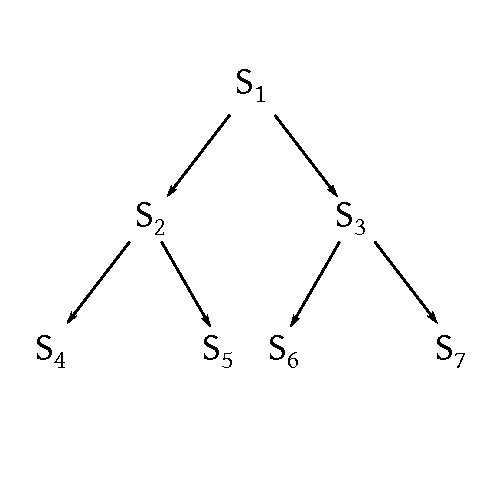
\includegraphics{img/searchtree.pdf}
    \caption{Binary search tree with sets of sets of clauses as nodes.}
    \label{fig:bintree_clauses}
  \end{center}
\end{figure}

This tree traversal can be implemented using activation literals and SAT solver assumption techniques.

If we want to evaluate the path $S_1 \land S_2 \land S_4$, we introduce a new activation literal $a_i$ for each set $S_i$ and use implication to (de)activate the clause:
%
\[
  (a_1 \implies S_1) \land (a_2 \implies S_2) \land (a_4 \implies S_4)
\]

Because each node itself is a conjunctive normal form, a set $S_i$ is the conjunction of its clauses giving us:
%
\[
  (a_1 \implies (c_1 \land c_2 \land c_3 \land \ldots)) \land
    (a_2 \implies (c_{10} \land c_{11} \land c_{12} \land \ldots)) \land
    (a_3 \implies (c_{20} \land c_{21} \land c_{22} \land \ldots)) \land
    \ldots
\]

This can be transformed to conjunctive normal form by resolving the clauses with the law of distributivity. In real-world implementations activation literals are represented as \emph{assumptions} in SAT solvers
to be able to drop their value for evaluation of the next search path (assumptions are described in section~\ref{sec:satsolvers-assumptions}).

For example the conjunctive normal form with boolean variables $v_1$ to $v_8$
%
\[
  (v_1 \lor \neg v_2) \land (\neg v_3 \lor \neg v_4 \lor v_5) \land
    (v_6 \lor v_7 \lor v_8)
\]

with activation literals $a_1$ to $a_3$
\[
  (a_1 \implies (v_1 \lor \neg v_2)) \land
    (a_2 \implies (\neg v_3 \lor \neg v_4 \lor v_5)) \land
    (a_3 \implies (v_6 \lor v_7 \lor v_8))
\]

resolved with the law of distributivity
\[
  (\neg a_1 \lor v_1 \lor \neg v_2) \land
    (\neg a_2 \lor \neg v_3 \lor \neg v_4 \lor v_5) \land
    (\neg a_3 \lor v_6 \lor v_7 \lor v_8)
\]

gives us a boolean expression in CNF.

\subsubsection{Algorithm}
\label{sec:activation-literals-algorithm}
%
\begin{description}
  \item[Initialization] Overlapping bits and the number of bit conditions are known.
    \begin{description}
      \item[Detect Overlapping Bits] Iterate over all bit conditions and store overlapping bit conditions.
      \item[Introduce new bit conditions] Introduce a new \texttt{SatCondition} object for every bit condition that will be used. A bit condition gets skipped, if this is not the first reference to an overlapping bit.
      \item[Setup Encoding] $7$ boolean variables per bit condition are requested from the SAT solver. The clauses given in Table~\ref{tab:simple-eval-clauses} are added.
      \item[Apply function to bitslices] Add all clauses which result from the function definition applied to this differential characteristic.
    \end{description}
  \item[Update BitCondition] The values of the bit conditions are known.
    \begin{description}
      \item[Set bit condition value] The assumptions resulting from the bit condition value are created. They are given in Table~\ref{tab:simple-eval-clauses}.
      \item[Run SAT solver] If the SAT solver returns satisfiability as result, the differential characteristic is satisfiable.
    \end{description}
\end{description}

\begin{table}[p]
  \begin{center}
    \begin{tabular}{cll}
      bit condition  & Setup Encoding (\gls{cnf})                        & Set bit condition value (assumptions) \\
    \hline
      \bc{\#}        & $(\neg a_1 \lor z) \land (\neg a_1 \lor \neg z)$  & $a_1 = 1$ \\
      \bc{0}         &                                                   & $z = 0, z^* = 0$ \\
      \bc{u}         &                                                   & $z = 1, z^* = 0$ \\
      \bc{3}         &                                                   & $z^* = 0$ \\
      \bc{n}         &                                                   & $z = 0, z^* = 1$ \\
      \bc{5}         &                                                   & $z = 0$ \\
      \bc{x}         &                                                   & $a_2 = 1, a_5 = 1$ \\
      \bc{7}         & $(\neg a_2 \lor \neg z \lor \neg z^*)$            & $a_2 = 1$ \\
      \bc{1}         &                                                   & $z = 1, z^* = 1$ \\
      \bc{-}         &                                                   & $a_3 = 1, a_4 = 1$ \\
      \bc{A}         &                                                   & $z = 1$ \\
      \bc{B}         & $(\neg a_3 \lor z \lor \neg z^*)$                 & $a_3 = 1$ \\
      \bc{C}         &                                                   & $z^* = 1$ \\
      \bc{D}         & $(\neg a_4 \lor \neg z \lor z^*)$                 & $a_4 = 1$ \\
      \bc{E}         & $(\neg a_5 \lor z \lor z^*)$                      & $a_5 = 1$ \\
      \bc{?}         &                                                   &
    \end{tabular}
    \caption[Activation literals clauses and assumptions]{
        Activation literals clauses and assumptions.
        Be aware that all activation literals $a_i$ must be set to false,
        if not stated otherwise.
    }
    \label{tab:simple-eval-clauses}
  \end{center}
\end{table}

\subsubsection{Discussion}
\label{sec:activation-literals-discussion}
%
The number of activation literals is linear to the number of nodes within the search tree. Every node represents one of sixteen possible bit conditions. However not all bit conditions have to be encoded using activation literals\footnote{This approach would obviously possible but less efficient}.

The bit conditions \bc{\#}, \bc{0}, \bc{u}, \bc{3}, \bc{n}, \bc{5}, \bc{1}, \bc{A}, \bc{C} and \bc{?} can directly be represented by assignments. The $6$ bit conditions \bc{x}, \bc{7}, \bc{-}, \bc{B}, \bc{D} and \bc{E} use the $\lor$ operator which has to be designed by explicit clauses.

For one additional bit condition we need $6$ clauses, $5.6875$ assumptions ($21$ assumptions from the right column in Table~\ref{tab:simple-eval-clauses} and $70$ activation literals set to false divided by $16$ bit conditions) and $7$ variables in average. Due to the high number of assumptions it was estimated that another approach would be more successful and no implementation is provided. No statistics are available. But this estimation is biased and requires further investigation in follow-up scientific work.

\subsection{Approach \#3: Assumption-based encodings}
\label{sec:encoding:assumption-encodings}
%
Like the activation literals approach in section~\ref{sec:encoding:activation-literals}, these approaches uses assumption to enable automated search. They do not use activation literals and only focus on efficient usage of assumptions. Three different approaches are taken which vary in the number of variables, clauses and assumptions.

\subsection{Exhaustive Encoding}
\label{sec:encoding:exhaustive}
%
The Exhaustive encoding consists of $17$ boolean variables per bit condition. Exhaustive refers to the large number of boolean variables. Each differential state gets its own assumption variable.

\subsubsection{Algorithm}
\label{sec:exhaustive-algorithm}
%
\begin{description}
  \item[Initialization] Overlapping bits and the number of bit conditions are known.
    \begin{description}
      \item[Detect Overlapping Bits] Iterate over all bit conditions and store overlapping bit conditions.
      \item[Introduce new bit conditions] Introduce a new \texttt{SatCondition} object for every bit condition that will be used. A bit condition gets skipped, if this is not the first reference to an overlapping bit.
      \item[Setup Encoding] $17$ boolean variables per bit condition are requested from the SAT solver. The clauses given below this algorithm are added.
      \item[Apply function to bitslices] Add all clauses which result from the function definition applied to this differential characteristic.
    \end{description}
  \item[Update BitCondition] The values of the bit conditions are known.
    \begin{description}
      \item[Set bit condition value] Given a bit condition $T$, the corresponding assumption $z_T$ is set to true.
      \item[Run SAT solver] If the SAT solver returns satisfiability as result, the differential characteristic is satisfiable.
    \end{description}
\end{description}

\begin{align*}
  z_\# & = \neg z_\#                          & \text{1 XOR clause or 2 CNF clauses} \\
  z_0  & = \neg z \land \neg z^*              & \text{3 CNF clauses} \\
  z_u  & = z \land z^*                        & \text{3 CNF clauses} \\
  z_3  & = \neg z^*                           & \text{1 XOR clause or 2 CNF clauses} \\
  z_n  & = \neg z^* \land z^*                 & \text{3 CNF clauses} \\
  z_5  & = \neg z                             & \text{1 XOR clause or 2 CNF clauses} \\
  z_X  & = z \oplus z^*                       & \text{4 CNF clauses} \\
  z_7  & = \neg z \lor \neg z^*               & \text{4 CNF clauses} \\
  z_1  & = z \land z^*                        & \text{3 CNF clauses} \\
  z_-  & = \neg(z \oplus z^*)                 & \text{1 XOR clauses or 4 CNF clauses} \\
  z_A  & = z                                  & \text{1 XOR clauses or 2 CNF clauses} \\
  z_B  & = \neg((z \land z^*) \oplus z^*)     & \text{4 CNF clauses} \\
  z_C  & = z^*                                & \text{1 XOR clause or 2 CNF clauses} \\
  z_D  & = \neg(z \land z^* \lor z)           & \text{4 CNF clauses} \\
  z_E  & = ((z\land z^*) \oplus z \oplus z^*) & \text{4 CNF clauses} \\
\end{align*}

The bit condition $?$ is skipped, because it does not constrain the boolean system in any way.

\subsubsection{Discussion}
\label{sec:exhaustive-discussion}
%
For this encoding obviously some reductions can be applied if one bit condition is a superset of another one (as can be seen in the lattice of Figure~\ref{fig:bitconditions-lattice}). Those reductions have been applied in the following encodings. Because this encoding has an extraordinary high number of variables, we assume that this encoding will not perform good in any case. Because no implementation was provided, no statistics are available.

\subsection{Reduced Encoding}
\label{sec:encoding:reduced-encoding}
%
The following approach was initially proposed by Martin Schläffer. It takes $9$ variables for each bit condition.

\subsubsection{Algorithm}
\label{sec:reduced-encoding-algorithm}
%
The 9 variables are denoted as $z, z^*, z_A, z_B, z_C, z_D, z_E, z_x$ and $z_1$.
%
\begin{description}
  \item[Initialization] Overlapping bits and the number of bit conditions are known.
    \begin{description}
      \item[Detect Overlapping Bits] Iterate over all bit conditions and store overlapping bit conditions.
      \item[Introduce new bit conditions] Introduce a new \texttt{SatCondition} object for every bit condition that will be used. A bit condition gets skipped, if this is not the first reference to an overlapping bit.
      \item[Setup Encoding] $9$ boolean variables per bit condition are requested from the SAT solver. The clauses given below this algorithm are added.
      \item[Apply function to bitslices] Add all clauses which result from the function definition applied to this differential characteristic.
    \end{description}
  \item[Update BitCondition] The values of the bit conditions are known.
    \begin{description}
      \item[Set bit condition value] The assumptions resulting from the bit condition value are created. They are given in Table~\ref{tab:reduced-encoding-assumptions}.
      \item[Run SAT solver] If the SAT solver returns satisfiability as result, the differential characteristic is satisfiable.
    \end{description}
\end{description}

In the Setup Encoding step the following relations are defined for the variables:
\begin{align*}
  z_A & = z_1                   & \text{1 XOR clause or 2 CNF clauses} \\
  z_B & = z_1 \lor \neg z_1^*   & \text{3 CNF clauses} \\
  z_C & = z^*                   & \text{1 XOR clause or 2 CNF clauses} \\
  z_D & = \neg z \lor z^*       & \text{3 CNF clauses} \\
  z_E & = z \lor z^*            & \text{3 CNF clauses} \\
  z_X & = z \oplus z^*          & \text{1 XOR clause or 4 CNF clauses} \\
  z_1 & = z \land z^*           & \text{1 XOR clause or 3 CNF clauses} \\
\end{align*}

Recognize that $a = (b \land c)$ can be represented by 3 clauses in CNF using $(\neg a \lor c) \land (\neg a \lor b \lor \neg c) \land (a \lor \neg b \lor \neg c)$.
\begin{table}[p]
  \begin{center}
    \begin{tabular}{cll}
      bit condition  & Set bit condition value \\
    \hline
      \bc{\#}        & $z_1 = 1, z_x = 1$ \\
      \bc{0}         & $z_A = 0, z_C = 0$ \\
      \bc{u}         & $z_A = 1, z_C = 0$ \\
      \bc{3}         & $z_C = 0$ \\
      \bc{n}         & $z_A = 0, z_C = 0$ \\
      \bc{5}         & $z_A = 0$ \\
      \bc{x}         & $z_X = 1$ \\
      \bc{7}         & $z_1 = 0$ \\
      \bc{1}         & $z_1 = 1$ \\
      \bc{-}         & $z_X = 0$ \\
      \bc{A}         & $z_A = 1$ \\
      \bc{B}         & $z_B = 1$ \\
      \bc{C}         & $z_C = 1$ \\
      \bc{D}         & $z_D = 1$ \\
      \bc{E}         & $z_E = 1$ \\
      \bc{?}         & 
    \end{tabular}
    \caption{Assumptions for the Reduced encoding.}
    \label{tab:reduced-encoding-assumptions}
  \end{center}
\end{table}

\subsubsection{Discussion}
\label{sec:reduced-encoding-discussion}
%
One additional bit condition requires $9$ boolean variables, $20$ clauses and $1.25$ assumptions in average.
In our SHA-256 testcase it reached up to 177 iterations per second.

\subsection{Differential state encoding}
\label{sec:encoding:dse}
%
\subsubsection{Algorithm}
\label{sec:encoding:dse-algorithm}
%
The 4 variables are denoted as $z_A, z_B, z_C$ and $z_D$. They exactly correspond to one of the cases $\{(0, 0), (0, 1), (1, 0), (1, 1)\}$ for the bits in the evaluation instances. $z_A$ corresponds to \bc{0}, $z_B$ is the same as \bc{n}, $z_C$ is \bc{u} and $z_D$ equals to \bc{1}. We require that only one of the cases is met in the Setup Encoding represented by 7 clauses.
%
\begin{description}
  \item[Initialization] Overlapping bits and the number of bit conditions are known.
    \begin{description}
      \item[Detect Overlapping Bits] Iterate over all bit conditions and store overlapping bit conditions.
      \item[Introduce new bit conditions] Introduce a new \texttt{SatCondition} object for every bit condition that will be used. A bit condition gets skipped, if this is not the first reference to an overlapping bit.
      \item[Setup Encoding] $4$ boolean variables per bit condition are requested from the SAT solver. The clauses given below this algorithm are added.
      \item[Apply function to bitslices] Add all clauses which result from the function definition applied to this differential characteristic.
    \end{description}
  \item[Update BitCondition] The values of the bit conditions are known.
    \begin{description}
      \item[Set bit condition value] The assumptions resulting from the bit condition value are created. They are given in Table~\ref{tab:dse-assumptions}.
      \item[Run SAT solver] If the SAT solver returns satisfiability as result, the differential characteristic is satisfiable.
    \end{description}
\end{description}

The Setup Encoding clauses can be represented by 1 XOR clause and 4 CNF clauses
\begin{alignat*}{4}
  (z_A      & \oplus    z_B & & \oplus    z_C & & \oplus    z_D & & ) \land \\
  (z_A      & \lor \neg z_B & & \lor \neg z_C & & \lor \neg z_D & & ) \land \\
  (\neg z_A & \lor      z_B & & \lor \neg z_C & & \lor \neg z_D & & ) \land \\
  (\neg z_A & \lor \neg z_B & & \lor      z_C & & \lor \neg z_D & & ) \land \\
  (\neg z_A & \lor \neg z_B)& & \lor \neg z_C & & \lor      z_D & & ) \\
\end{alignat*}

or 7 CNF clauses:
\begin{alignat*}{4}
  (z_A & \lor           z_B & & \lor z_C       & & \lor z_D)      & & \land \\
  (z_A & \lor           z_B & & \lor \neg z_C  & & \lor \neg z_D) & & \land \\
  (z_A & \lor \neg      z_B & & \lor z_C       & & \lor \neg z_D) & & \land \\
  (z_A & \lor \neg      z_B & & \lor \neg z_C) & &                & & \land \\
  (\neg z_A & \lor      z_B & & \lor z_C       & & \lor \neg z_D) & & \land \\
  (\neg z_A & \lor      z_B & & \lor \neg z_C) & &                & & \land \\
  (\neg z_A & \lor \neg z_B) & &               & &                & & \\
\end{alignat*}

\begin{table}[p]
  \begin{center}
    \begin{tabular}{cll}
      bit condition  & Set bit condition value \\
    \hline
      \bc{\#}        & $z_A = 0, z_B = 0, z_C = 0, z_D = 0$ \\
      \bc{0}         & $z_A = 1$ \\
      \bc{u}         & $z_C = 1$ \\
      \bc{3}         & $z_B = 0, z_D = 0$ \\
      \bc{n}         & $z_B = 1$ \\
      \bc{5}         & $z_C = 0, z_D = 0$ \\
      \bc{x}         & $z_A = 0, z_D = 0$ \\
      \bc{7}         & $z_D = 0$ \\
      \bc{1}         & $z_D = 1$ \\
      \bc{-}         & $z_B = 0, z_C = 0$ \\
      \bc{A}         & $z_A = 0, z_D = 0$ \\
      \bc{B}         & $z_B = 0$ \\
      \bc{C}         & $z_A = 0, z_C = 0$ \\
      \bc{D}         & $z_C = 0$ \\
      \bc{E}         & $z_A = 0$ \\
      \bc{?}         & 
    \end{tabular}
    \caption{Assumptions for the Differential State encoding.}
    \label{tab:dse-assumptions}
  \end{center}
\end{table}

\subsubsection{Discussion}
\label{sec:dse-discussion}
%
One additional bit condition requires $4$ boolean variables, $7$ clauses and $1.5$ assumptions in average. The open question is which one is worse: a high number of clauses or a high number of variables. A high number of variables might segment the search space for the SAT solver which leads to fast evaluation. In this implementation further analysis is required whether this might happen for this architecture.


\chapter{Future work}
\label{chap:next}
\section{Results and comparison}
%
% REMARK. testcases are run for about 900 seconds. iter/sec was taken from the last entry
%         started with ./nltool -i ../hash/sha2/chars/sha256/startchars/27-t10.xml
%         SAT_EXPLICIT_SOLUTION must be disabled in every branch.
%
%\begin{table}[t]
\begin{sidewaystable}
 \begin{center}
  \begin{tabular}{lccccc}
                               & \multicolumn{3}{c}{1 additional bit condition requires in average} & \\
   Approach                    & boolean vars & clauses & assumptions   & performance \\
  \hline
   % lp/sat-se: Info: seed: 2578791537 time: 886 iterations/sec: 0 iterations: 568 stack_size: 4 contr: 38 restarts: 1 minfree: 105 absminfree: 105 credits: 9962 phase: 0 found: 0 smax: 9 complete: 0/0 
   % lp/sat-se: Info: seed: 2578791537 time: 888 iterations/sec: 0 iterations: 569 stack_size: 4 contr: 38 restarts: 1 minfree: 105 absminfree: 105 credits: 9962 phase: 0 found: 0 smax: 9 complete: 0/0 
   Simple evaluation           & $2.0$        & $1.375$ & $0$           & $0$ iter/sec \\
   % lp/sat-al: Info: seed: 1124351917 time: 887 iterations/sec: 23 iterations: 130 stack_size: 0 contr: 3 restarts: 63 minfree: 160 absminfree: 44 credits: 9997 phase: 0 found: 0 smax: 3 complete: 0/0 
   % lp/sat-al: Info: seed: 1124351917 time: 889 iterations/sec: 23 iterations: 38 stack_size: 1 contr: 0 restarts: 64 minfree: 315 absminfree: 44 credits: 10000 phase: 0 found: 0 smax: 1 complete: 0/0 
   %
   % lp/sat-al: Info: seed: 1124351917 time: 895 iterations/sec: 23 iterations: 113 stack_size: 4 contr: 0 restarts: 65 minfree: 197 absminfree: 44 credits: 10000 phase: 0 found: 0 smax: 4 complete: 0/0 
   % lp/sat-al: Info: seed: 1124351917 time: 897 iterations/sec: 23 iterations: 61 stack_size: 1 contr: 0 restarts: 66 minfree: 276 absminfree: 44 credits: 10000 phase: 0 found: 0 smax: 1 complete: 0/0
   Activation literals         & $7.0$        & $6$     & $5.6875$      & $\approx23$ iter/sec \\
   Exhaustive encoding         & $17$         & $46$    & $1$           & N/A \\
   % lp/sat-re: Info: seed: 843358102 time: 886 iterations/sec: 11 iterations: 146 stack_size: 3 contr: 5 restarts: 33 minfree: 159 absminfree: 51 credits: 9995 phase: 0 found: 0 smax: 4 complete: 0/0 
   % lp/sat-re: Info: seed: 843358102 time: 888 iterations/sec: 11 iterations: 171 stack_size: 1 contr: 10 restarts: 33 minfree: 151 absminfree: 51 credits: 9990 phase: 0 found: 0 smax: 4 complete: 0/0 
   % lp/sat-re: Info: seed: 843358102 time: 890 iterations/sec: 11 iterations: 193 stack_size: 4 contr: 10 restarts: 33 minfree: 151 absminfree: 51 credits: 9990 phase: 0 found: 0 smax: 4 complete: 0/0 
   %
   % lp/sat-re: Info: seed: 843358102 time: 899 iterations/sec: 11 iterations: 315 stack_size: 0 contr: 24 restarts: 33 minfree: 118 absminfree: 51 credits: 9976 phase: 0 found: 0 smax: 5 complete: 0/0 
   % lp/sat-re: Info: seed: 843358102 time: 901 iterations/sec: 11 iterations: 25 stack_size: 1 contr: 0 restarts: 34 minfree: 320 absminfree: 51 credits: 10000 phase: 0 found: 0 smax: 1 complete: 0/0 
   % lp/sat-re: Info: seed: 843358102 time: 903 iterations/sec: 11 iterations: 59 stack_size: 1 contr: 0 restarts: 34 minfree: 286 absminfree: 51 credits: 10000 phase: 0 found: 0 smax: 1 complete: 0/0 
   Reduced encoding            & $9$          & $20$    & $1.25$        & $\approx11$ iter/sec \\
   % lp/sat-dse: Info: seed: 1503521737 time: 894 iterations/sec: 7 iterations: 217 stack_size: 8 contr: 2 restarts: 12 minfree: 162 absminfree: 18 credits: 9998 phase: 0 found: 0 smax: 8 complete: 0/0
   % lp/sat-dse: Info: seed: 1503521737 time: 896 iterations/sec: 7 iterations: 237 stack_size: 4 contr: 10 restarts: 12 minfree: 159 absminfree: 18 credits: 9990 phase: 0 found: 0 smax: 8 complete: 0/0
   % lp/sat-dse: Info: seed: 1503521737 time: 898 iterations/sec: 7 iterations: 262 stack_size: 2 contr: 13 restarts: 12 minfree: 159 absminfree: 18 credits: 9987 phase: 0 found: 0 smax: 8 complete: 0/0
   % lp/sat-dse: Info: seed: 1503521737 time: 900 iterations/sec: 7 iterations: 283 stack_size: 3 contr: 13 restarts: 12 minfree: 159 absminfree: 18 credits: 9987 phase: 0 found: 0 smax: 8 complete: 0/0
   % lp/sat-dse: Info: seed: 1503521737 time: 902 iterations/sec: 7 iterations: 302 stack_size: 1 contr: 16 restarts: 12 minfree: 159 absminfree: 18 credits: 9984 phase: 0 found: 0 smax: 8 complete: 0/0
   Differential state encoding & $4$          & $7$     & $1.5$         & $\approx7$ iter/sec \\
  \end{tabular}
  \caption[All encodings in comparison]{
    All encodings in comparison.
    The number of variables and clauses is not important in the first place, but will influence the SAT solvers performance.
    A small number of assumptions is desirable in any case.
  }
  \label{tab:encoding-cmp}
 \end{center}
%\end{table}
\end{sidewaystable}

Simple evaluation obviously has the worst performance. Destroying and building the SAT solver takes a lot of time and slows down the automated search. The advantage of this approach comes into play, when the evaluated differential characteristic is very large. However this size is not within the scope for SAT-based attacks of hash algorithms.

The approaches for Activation literals, Reduced encoding and Differential state encoding all seem interesting and perform very good. Further study is advised to improve the speed by studying the recurring structures due to assigned bit conditions.

\section{Propagation}
%
The propagation in the automated search improved previous implementation, because overlapping bits are detected and considered. Therefore the implementation scales better for larger sizes, because invalid paths are eliminated faster. Figure~\ref{fig:sat-propagation} can directly be compared to the propagation diagrams given in~\cite{Cry16}.
%
\begin{figure}[t]
 \begin{center}
  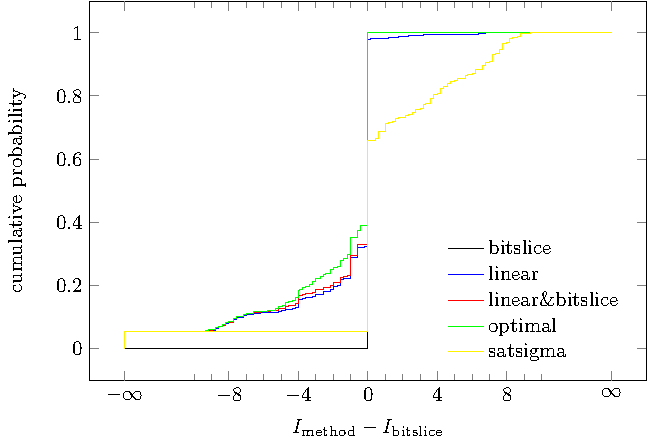
\includegraphics{img/propagation.pdf}
  \caption[Comparison of propagation methods.]{Comparison of propagation methods. Higher values mean better propagation.}
  \label{fig:sat-propagation}
 \end{center}
\end{figure}

\section{Implementation-dependent improvements}
%
\begin{itemize}
  \item Tests shall be made also with different state-of-the-art SAT solvers from different families of the DPLL algorithm such that comparison is possible.
  \item An implementation of the activation literal approach is desirable.
  \item The truth table is a bottleneck of the Initialization step. Tests are required whether approaches like Tseitin's Definitional Normal Form perform better as discussed in~\cite{Sat03}.
  \item SAT solvers themselves propagate values in their evaluation. The same concept is desirable in \nltool. Strategies to put SAT solver technology directly into the framework shall be discussed.
  \item Any fast simplification algorithms for boolean equations are of interest. In the initialization step all clauses are already known. Performing a simplification algorithm especially to the clauses of the primitive functions might lead to a speedup. Karnaugh maps, the Quine-McCluskey algorithm and the Espresso algorithm shall be considered. Simplification algorithms have been implemented by Akawat Homsirikamol et~al.~\cite{Cry04} with HDL in the Quartus II software.
\end{itemize}

\section{Independent approaches}
%
\begin{itemize}
  \item SMT solvers and STP allow a more powerful encoding of the problem to solve. This deprecates the usage of truth tables and encodings. A comparison is of interest.
\end{itemize}


\appendix
\chapter{CNF transformations for boolean equations}
\label{appendix:cnf}
Table~\ref{tab:cnf-transformations} lists CNF transformations. The encodings mentioned in this document were described with general boolean algebra, but SAT solvers restrict the input to be in conjunctive normal form. \cmsat{} also allows us to XOR clauses. We provide only shorter XOR clauses; others are omitted. The table lists transformations to achieve CNF.

\begin{sidewaystable}
  \begin{center}
    \begin{tabular}{ccc}
      boolean expression   & CNF and XOR clauses & CNF clauses \\
     \hline
      $a = b$              & $\neg (a \oplus b)$ & $(a \lor \neg b) \land (\neg a \lor b)$ \\
      $a \oplus b$         & $a \oplus b$        & $(a \lor b) \land (\neg a \lor \neg b)$ \\
      $a = (b \land c)$    &                     & $(a \lor \neg b \lor \neg c) \land (\neg a \lor b) \land (\neg a \lor c)$ \\
      $a = (b \lor c)$     &                     & $(\neg \lor b \lor c) \land (a \lor \neg b) \land (a \lor \neg c)$ \\
      $a = (b \oplus c)$   &                     & $(\neg a \lor b \lor c) \land (a \lor \neg b \lor c) \land (a \lor b \lor b \neg c) \land (\neg a \lor \neg b \lor \neg c)$ \\
      $a = (b \implies c)$ &                     & $(a \lor b \lor c) \land (\neg a \lor \neg b \lor c) \land (a \lor b \lor \neg c) \land (a \lor \neg b \lor \neg c)$ \\
    \end{tabular}
    \caption{CNF transformations.}
    \label{tab:cnf-transformations}
  \end{center}
\end{sidewaystable}


\hypersetup{colorlinks=true,linktoc=all,linkcolor=contr}

\printbibliography
\listofalgorithms
\listoffigures
\listoftables
\printindex

\end{document}
